% !TeX root = ../../../main.tex

The impact of intrinsic charm on hadron collider observables can be
assessed by studying  parton luminosities. Indeed, the
cross-section for hadronic processes at leading order is typically
proportional to an individual parton luminosity or linear combination
of parton luminosities.
%
Comparing parton luminosities determined
using our default \pdf set to those obtained imposing perturbative
charm (see SI Sect.~\ref{sec:ic/consistency}) provides a qualitative estimate of the
measurable impact of intrinsic charm. Of course this is then modified
by higher-order
perturbative corrections, which generally depend on more partonic
subchannels and thus on more luminosities.
%
In this section we illustrate this by considering the parton
luminosities that are relevant for the computation of the
$Z$+charm process in the \lhcb kinematics, see SI Sect.~\ref{sec:ic/zcharm}.

The parton luminosity without any restriction on the rapidity $y_X$ of the final state is
\begin{equation}
\label{eq:ic/lumi1D}
\mathcal{L}_{ab}(m_X)= \frac{1}{s}\int_{\tau}^1 \frac{dx}{x}f_a \left( x,m_X^2\right)
f_b\left( \tau/x,m_X^2\right) \, ,\qquad
\tau=\frac{m_X^2}{s} \, ,
\end{equation}
where $a,b$ label the species of incoming partons, $\sqrt{s}$ is the center-of-mass energy of
the hadronic collision, and $m_X$ is the final state invariant mass.
%
For the more realistic situation where the final state rapidity
is restricted, $y_\textrm{ min}\le y_X\le y_\textrm{ max}$,
Eq.~(\ref{eq:ic/lumi1D}) is modified as
\begin{equation}
\label{eq:ic/lumi1D_restricted}
\mathcal{L}_{ab}(m_X)= \frac{1}{s}\int_{\tau}^1 \frac{dx}{x}f_a \left( x,m_X^2\right)
f_b\left( \tau/x,m_X^2\right) \theta\left( y_X-y_\textrm{ min}  \right)
\theta\left( y_\textrm{ max}-y_X  \right)\, , 
\end{equation}
where $y_X = \left( \ln x^2/\tau \right) /2$.

We consider in particular the quark-gluon and the charm-gluon luminosities, defined as
\begin{equation}
\label{eq:ic/lumis}
\mathcal{L}_{qg}(m_X)\equiv \sum_{i=1}^{n_f} \left( \mathcal{L}_{q_ig}(m_X)+
\mathcal{L}_{\bar{q}_ig}(m_X) \right)\, , \quad
\mathcal{L}_{cg}(m_X)\equiv  \left( \mathcal{L}_{cg}(m_X)+
\mathcal{L}_{\bar{c}g}(m_X) \right)\, , 
\end{equation}
where $n_f$ is the number of active quark flavors for a given value of $Q=m_X$
with a maximum value of $n_f=5$.
%
These are the combinations that provide the leading contributions
respectively to the numerator ($\mathcal{L}_{cg}$) and the 
denominator
($\mathcal{L}_{qg}$) of  $\mathcal{R}_j^c$ in Eq.~(\ref{eq:ic/Rcj}). 

%%%%%%%%%%%%%%%%%%%%%%%%%%%%%%%%%%%%%%%%%%%%%%%%%%%%%%%%%%%%%%%%%%%
\begin{figure}[htbp]
  \begin{center}
    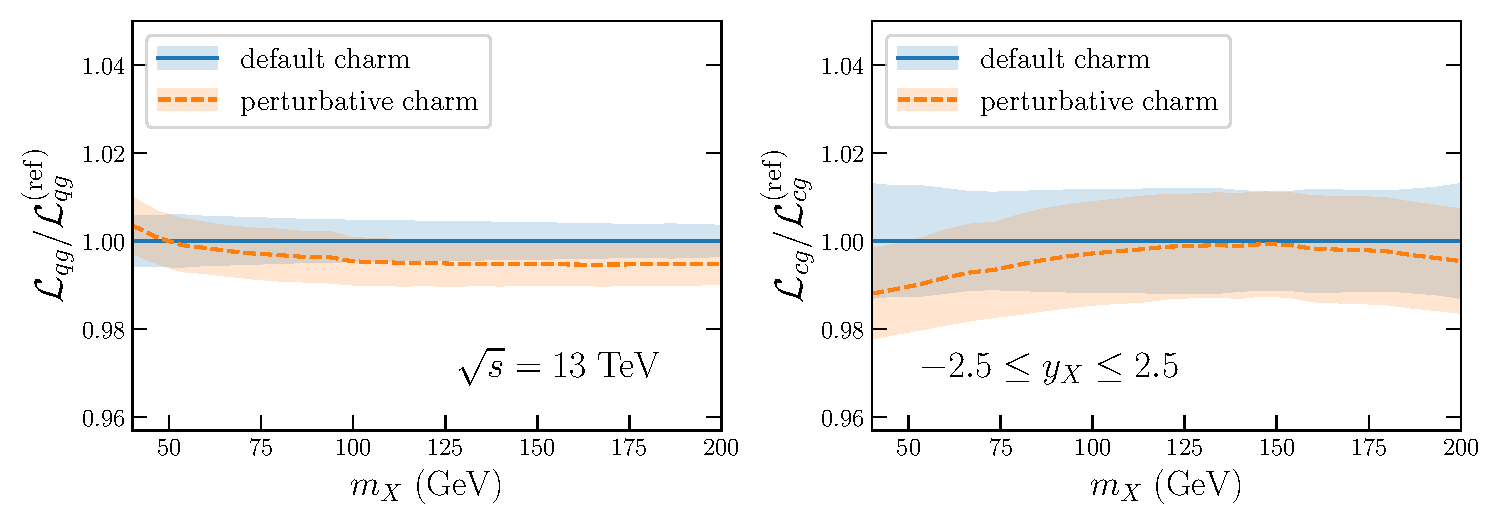
\includegraphics[width=0.99\linewidth]{ch-ic/cglumi-nnpdf40-ATLAScuts.pdf}
    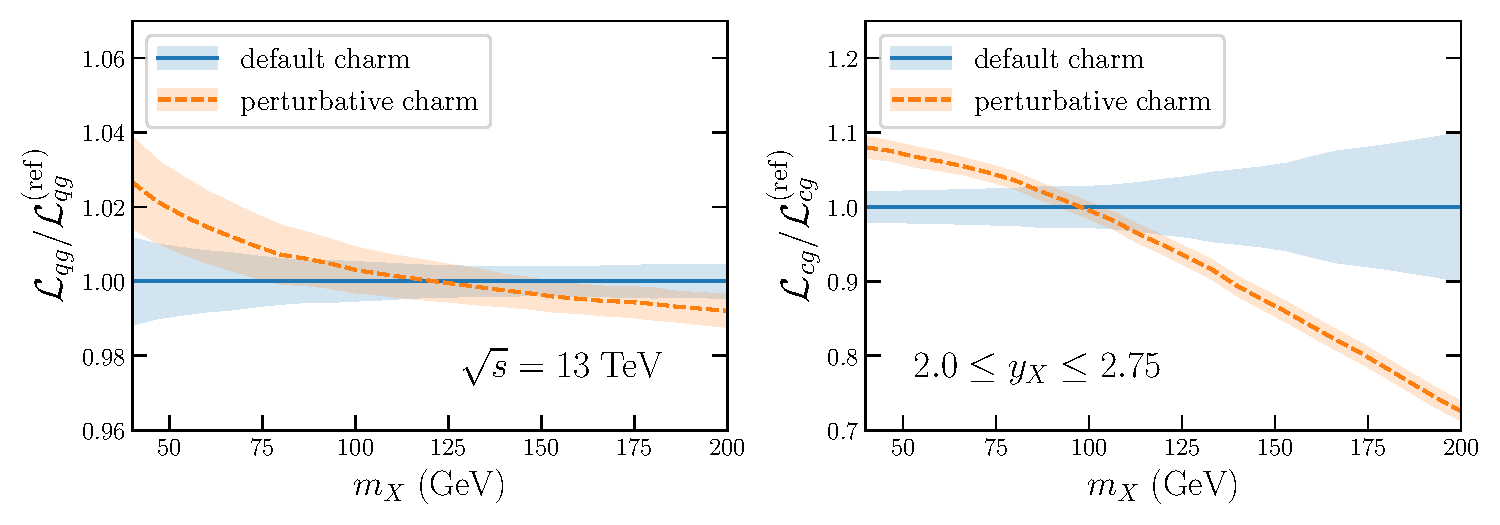
\includegraphics[width=0.99\linewidth]{ch-ic/cglumi-nnpdf40-LHCbcuts-central.pdf}
    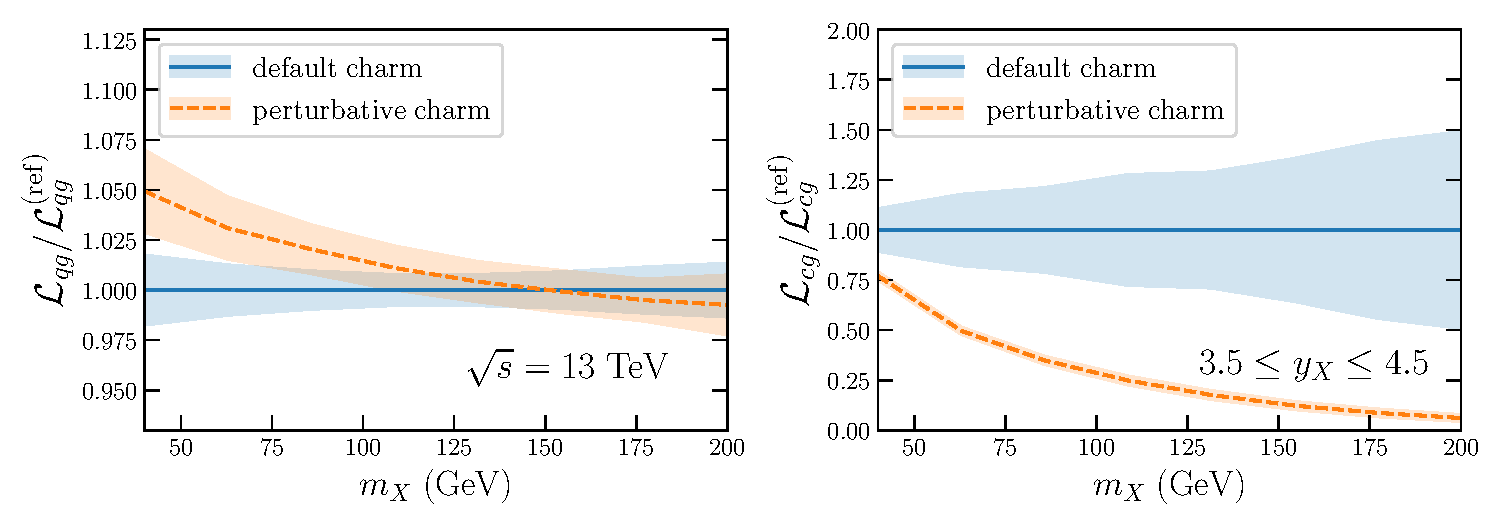
\includegraphics[width=0.99\linewidth]{ch-ic/cglumi-nnpdf40-LHCbcuts-forward.pdf}
    \caption{\small The quark-gluon (left) and charm-gluon (right)
      parton luminosities in the  $m_X$ region
      relevant for $Z$+charm production and  three different
      rapidity bins (see text). Results are shown both for our default charm
    \pdfs and for the variant with perturbative charm. 
  \label{fig:ic/charm_luminosities} }
\end{center}
\end{figure}
%%%%%%%%%%%%%%%%%%%%%%%%%%%%%%%%%%%%%%%%%%%%%%%%%%%%%%%%%%%%%%%%%

The luminosities are displayed in Fig.~\ref{fig:ic/charm_luminosities},
in the  invariant mass region,
$40~\textrm{ GeV}\le m_X \le 200~\textrm{ GeV}$ which is most relevant for
$Z$+charm production.
%
Results are shown 
for three different
rapidity bins, $-2.5 \le y_X \le 2.5$ (central production in \atlas and \cms),
$2.0 \le y_X \le 2.75$ (forward production, corresponding to the
central bin in \lhcb),
and $3.5 \le y_X \le 4.5$ (highly boosted production, corresponding to
the most forward bin in the \lhcb selection), as a ratio to our default case.

For central production it is clear that both the quark-gluon and
charm-gluon luminosities with our without intrinsic charm are very similar.
This means that central $Z$+charm production in this invariant mass
range is insensitive to intrinsic charm.
%
For forward production, corresponding to the  central \lhcb rapidity
bin, $2.0 \le y_X \le 2.75$, in the invariant mass region  $m_X\simeq
100$~GeV again there is little difference between results with or
without intrinsic charm, but as the invariant mass increases the
charm-gluon luminosity with intrinsic charm is significantly enhanced.
%
For very forward production, such as the highest rapidity bin of \lhcb,
$3.5 \le y_X \le 4.5$, the charm-gluon luminosity 
at $m_X \simeq 100$ GeV is enhanced  by a factor of about 4 in our
default result in comparison to the perturbative charm case, corresponding
to a $\simeq 3\sigma$ difference in units of the \pdf uncertainty,
consistently with the behavior observed for the 
$\mathcal{R}_j^c$ observable in Fig.~\ref{fig:ic/Zc}~(top left) in the
most forward rapidity  bin.
%
This observation provides a qualitative explanation of
the results of SI Sect.~\ref{sec:ic/zcharm}.

